\documentclass[10pt, a4paper]{article}
\usepackage[utf8]{inputenc}
\usepackage[frenchb]{babel}
\usepackage[OT1]{fontenc}
\usepackage{amsfonts, amsmath, amssymb, amsthm, dsfont, amsthm}
\usepackage{a4wide}
\usepackage[dvipsnames]{xcolor}
\usepackage{tikz} 
\usetikzlibrary{arrows,positioning,shapes}

\title{\textbf{Lab Report} \\ Week of 12/01/2016}
%\author{Olivier \textsc{Mangin}}
%\date{\today}

\definecolor{main}{named}{BurntOrange}
\definecolor{second}{named}{RoyalBlue}
%\newcommand{\maincolor}{orange}
%\newcommand{\secondcolor}{orange!20}
\newcommand{\strong}[1]{\textcolor{main}{\textbf{#1}}}
\newcommand{\stronger}[1]{\textcolor{second}{\textbf{#1}}}
\newcommand{\colored}[1]{\textcolor{main}{#1}}

% Affichage du titre avec les numéro et date de la semaine
\newcommand{\titre}[2]{
\noindent
\hspace{-10pt}
\begin{tabular}{lr}
  \hspace{0.58\textwidth} & \hspace{0.4\textwidth} \\
  \strong{\huge Lab Report} & \textbf{\Large #1} \medskip \\
  \textbf{\Large Name \& Roll} & {\large #2} ~\\
\end{tabular}

\vspace{20pt}
}

% Encadré ``En bref'' réumant les avancées et problèmes de la semaine
\newenvironment{enbref}{
\noindent\fcolorbox{main}{main}{
\begin{minipage}{\textwidth}
\textcolor{white}{\textbf{\large }}
\end{minipage}
} \\

}{
\begin{center}
  \strong{ \rule[2mm]{\textwidth}{3pt} }
\end{center}
\vspace*{-20pt}
}

% Affichage d'un titre de rubrique
\newcommand{\rubrique}[1]{
  \bigskip
  \begin{center}
  \begin{minipage}{\textwidth}
    \noindent\strong{{\large #1} \\
      \rule[2mm]{\textwidth}{1pt} }
  \end{minipage}
  \end{center}
  \vspace*{-20pt}
}

% Symbole utilisé en début de ligne des éléments
\newcommand{\doublerect}{
\begin{tikzpicture}
  \fill[color=main] (0,0) rectangle (4pt,-4pt);
  \fill[color=second] (2pt,-2pt) rectangle (6pt,-6pt);
\end{tikzpicture}
}

% Affichage d'un titre d'élément
\newcommand{\element}[1]{
  \medskip
  \noindent\textcolor{second}{ \doublerect \textbf{#1}}
}

% Pour les lectures, petit raccourci pour mettre en avant le niveau
% de lecture d'un article.
\newcommand{\lu}{\strong{[Lu]} }
\newcommand{\parcouru}{\strong{[Parcouru]} }
\newcommand{\alire}{\strong{[A lire]} }
\newcommand{\presentation}{\strong{[Présentation]} }
\newcommand{\keynote}{\strong{[Keynote]} }



\usepackage[pdfauthor={Name}, pdftitle={Weekly}, pdfsubject={Week 1}, pdfkeywords={},colorlinks=true,urlcolor=black,linkcolor=black, citecolor=black]{hyperref}
\usepackage{listings}
\usepackage{subfig}
\usepackage{graphicx}
\lstset{%
language=Matlab,
frame=single,
%numbers=left,
%numberstyle=\footnotesize,
%tabsize=2,
keepspaces=true,
columns=fullflexible,
basicstyle=\ttfamily\scriptsize,
keywordstyle=\color{blue}
}


\begin{document}

\renewcommand{\labelitemi}{\textcolor{main}{\small $\blacktriangleright$}}
\renewcommand{\labelitemii}{\textcolor{second}{\scriptsize \textbullet}}

\titre{Week 2}{30/01/2017}

\begin{enbref}
\element{Title}
\begin{itemize}
\item Draw a line in OpenGL and Matlab using:\\
1). Basic Digital Differential Analyzer (DDA) Algorithm (both Simple and Symmetric DDA)\\
2). Bresenham’s mid-point Line Drawing Algorithm
\end{itemize}
\medskip

%\element{Problèmes rencontrés}
%\begin{itemize}
%\item Néant.
%\end{itemize}
\end{enbref}

%\rubrique{Lectures}
%Néant.
%\element{\lu ... \cite{...}}

\rubrique{Procedure}
\vspace{0.5mm} \flushleft

\element {OpenGL}

\vspace{0.5mm} \flushleft
1). Draw a line using simple and symmetric DDA Line Algorithm.
\begin{itemize}
\item Create a C file and name it as \textit{dda\_lines.c}.

\item Define global variables to store coordinates of points of a line and option to choose between Simple and Symmetric DDA.

\item Following algorithm to compute incremental values of x and y in Simple DDA:

\begin{lstlisting}
length = abs(x_2-x_1);
if(length < abs(y_2-y_1))
	length = abs(y_2-y_1);
x_increment = (x_2-x_1)/length;
y_increment = (y_2-y_1)/length;
\end{lstlisting}

\item Following algorithm to compute incremental values of x and y in Symmetric DDA:

\begin{lstlisting}
x_increment = x_2-x_1 ;
y_increment = y_2-y_1 ;
while(abs(x_increment)>=1 || abs(y_increment)>=1)
{
	x_increment /= 2;
	y_increment /= 2;
}
\end{lstlisting}

\item Following algorithm to plot points in Simple and Symmetric DDA:

\begin{lstlisting}
x = x_1;
y = y_1;
while x < x_2
begin
	plot(round(x),round(y));
	x = x + x_increment;
	y = y + y_increment;
end
\end{lstlisting}

\item Following is the final code for Simple and Symmetric DDA Line Algorithm:
\begin{lstlisting}
#include <stdio.h>
#include <math.h>
#include <GL/glut.h>

double x_1 , x_2 , y_1 , y_2 , x_increment , y_increment ;
double length ;

displayLine(void)
{
	glClearColor(1,1,1,1);
	glClear(GL_COLOR_BUFFER_BIT | GL_DEPTH_BUFFER_BIT);
	glBegin(GL_LINES);
                glColor3f(0.0f, 0.0f, 0.0f);
                glVertex2f(0.0f,1.0f);
                glVertex2f(0.0f,-1.0f);
                glVertex2f(1.0f,0.0f);
                glVertex2f(-1.0f,0.0f);
        glEnd();
	glBegin(GL_LINE_STRIP);
	double x = round(x_1);
	double y = round(y_1);
	while(x <= x_2)
	{
		double xf = floor(x);
		double yf = floor(y);
		xf/=100;
		yf/=100;
		glVertex3f(xf,yf,1.0f);
		x += x_increment;
		y += y_increment;
	}
	glEnd();
	glFlush();
	glutSwapBuffers();
}

int main(int argc, char const *argv[])
{
	int flag=0;
	printf("Enter  the  coordinates  of first point  : ");
	scanf("%lf %lf",&x_1,&y_1);
	printf("Enter  the  coordinates  of Second point : ");
	scanf("%lf %lf",&x_2,&y_2);
	printf("Enter choice\n\t1 : Draw Line using simple DDA\n\t2 : Draw Line using Symmetric DDA\n");
	printf("Your choice : ");
	scanf("%d\n",&flag);
	glutInit(&argc,argv);
	glutInitDisplayMode(GLUT_DOUBLE | GLUT_RGB | GLUT_DEPTH);

	if(flag==1)
	{
		length = abs(x_2-x_1);
		if(length < abs(y_2-y_1))
			length = abs(y_2-y_1);
		x_increment = (x_2-x_1)/length;
		y_increment = (y_2-y_1)/length;
		glutCreateWindow("Demonstrating Simple DDA");
		
	}
	else if(flag==2)
	{
		x_increment = x_2-x_1 ;
		y_increment = y_2-y_1 ;
		while(abs(x_increment)>=1 || abs(y_increment)>=1)
		{
			x_increment /= 2;
			y_increment /= 2;
		}
		glutCreateWindow("Demonstrating Symmetric DDA");
	}
	else 
	{
		printf("Please try with correct input\n");
		exit(1);
	}
	glutDisplayFunc(displayLine);
	glutMainLoop();
	return 0;
}
\end{lstlisting}

\vspace{0.5mm}

\item Compile and run the executable file in terminal by typing in the following commands : \\

\vspace{0.5mm} \flushleft

\textit{(a)\hspace{2mm} gcc dda\_lines.c -lGL -lGLU -lglut -lm} \\
\textit{(b)\hspace{2mm} ./a.out}
\vspace*{1\baselineskip} 
\end{itemize}

2). Draw a line using Bresenham’s Line Drawing Algorithm :
\begin{itemize}
\item Create a C file and name it as \textit{bresenhams\_line.c}.

\item Define global variables to define coordinates of line and flag to find octant for line.

\item Following algorithm to compute values for coordinates of line:

\begin{lstlisting}
x := x_1;
y := y_1;
dx := x_2-x_1;
dy := y_2-y_1;
d := 2dy - dx;
while x < x_2
begin
	plot(x,y);
	if d<=0 /* Choose E */
		d = d + 2dy;
	else
	/* Choose NE */
		d = d + 2(dy - dx);
	y = y + 1;
	endif
	x = x + 1;
end
\end{lstlisting}

\item Following is the final code for Bresenham’s Line Drawing Algorithm:
\begin{lstlisting}
#include <stdio.h>
#include <math.h>
#include <GL/glut.h>
int x_1 , x_2 , y_1 , y_2 , flag , y_increment , d , d1 , d2 ;

void displayLine(void)
{
	glClearColor(1,1,1,1);
	glClear(GL_COLOR_BUFFER_BIT | GL_DEPTH_BUFFER_BIT);
	glBegin(GL_LINES);
                glColor3f(0.0f, 0.0f, 0.0f);
                glVertex2f(0.0f,1.0f);
                glVertex2f(0.0f,-1.0f);
                glVertex2f(1.0f,0.0f);
                glVertex2f(-1.0f,0.0f);
        glEnd();
	glBegin(GL_LINE_STRIP);
	glColor3f(0,0,0);
	double x = x_1, y = y_1;
	while(x < x_2)
	{
		glVertex3f(x/100.0,y/100.0,1.0f);
		if(d<=0)
			d += d1;
		else
		{
			d += d2;
			
			if(flag)
				y += y_increment;
			else
				x++;
		}
		if(flag)
			x++;
		else
			y += y_increment;
	}
	glEnd();
	glFlush();
	glutSwapBuffers();
}

int main(int argc, char **argv)
{
	printf("Enter  the  coordinates  of first point  : ");
	scanf("%d %d",&x_1,&y_1);
	printf("Enter  the  coordinates  of Second point : ");
	scanf("%d %d",&x_2,&y_2);
	glutInit(&argc, argv);
	glutInitDisplayMode(GLUT_DOUBLE | GLUT_RGB | GLUT_DEPTH);
	double slope = (y_2-y_1)/(x_2-x_1);
	if(slope <=1 && x_1 >=0 && x_2 >= 0 && y_1 >=0 && y_2 >= 0)
	{
		int dx = x_2-x_1;
		int dy = abs(y_2-y_1);
		if(y_2 < y_1)
			y_increment = -1;
		else
			y_increment = 1;
		if(dy>dx)
		{
			flag = 0;
			d = 2*dx - dy;
			d1 = 2*dx;
			d2 = 2*(dx-dy);
		}
		else
		{
			flag = 1;
			d = 2*dy - dx;
			d1 = 2*dy;
			d2 = 2*(dy-dx);
		}
	}
	else 
	{
		printf("Please enter the point  in first octant only\n");
		exit(1);
	}
	glutCreateWindow("Bresenham Line Drawing");
	glutDisplayFunc(displayLine);
	glutMainLoop();
	return 0;
}
\end{lstlisting}

\vspace{0.5mm}

\item Compile and run the executable file in terminal by typing in the following commands :

\vspace{0.5mm} \flushleft

\textit{(a)\hspace{2mm} gcc bresenhams\_line.c -lGL -lGLU -lglut -lm}\\
\textit{(b)\hspace{2mm} ./a.out}
\vspace*{3\baselineskip}
\end{itemize}

\element {MatLab}\\
1). Draw a line using Simple and Symmetric DDA Algorithm :
\begin{itemize}

\item Open a new Script and contruct a function dda\_lines(flag). The flag is passed as an argument,
which is 0 for Simple DDA and 1 for Symmetric DDA. The script prompts user for coordinates of the
starting and ending points of the line.

\item Following is the Matlab Script Code for DDA Algorithm :
\begin{lstlisting}
function [] = dda_lines(flag)
	x1 = input("Enter x-coordinate of first Point  : ");
	y1 = input("Enter y-coordinate of first Point  : ");
	x2 = input("Enter x-coordinate of second Point : ");
	y2 = input("Enter y-coordinate of second Point : ");
	dx = x2-x1;
	dy = y2-y1;
	if flag==0
		
		length = abs(x2-x1);
		
		if length < abs(y2-y1)
			length = abs(y2-y1);
		end
		
		dx = dx./length;
		dy = dy./length;
	end

	if flag==1
		while abs(dx)>=1 | abs(dy)>=1
			dx = dx./2;
			dy = dy./2;
		end
	end

	x = x1;
	y = y1;

	px = [x];
	py = [y];
	
	while x<x2
		x = x+dx;
		y = y+dy;
		px = [px round(x)];
		py = [py round(y)];
	end
	plot(px,py);
\end{lstlisting}
\vspace*{1\baselineskip}
\end{itemize}

2). Draw a Line using Bresenham’s Line Drawing Algorithm:

\begin{itemize}

\item Open a new Script and contruct a function bresenhams\_line(). The script prompts user for input of the starting and ending point\'s coordinates of the line.

\item Following is the Matlab Script Code for Bresenham’s Line Drawing Algorithm :
\begin{lstlisting}

function [] = bresenhams_line()
	x1 = input("Enter x-coordinate of first Point  : ");
	y1 = input("Enter y-coordinate of first Point  : ");
	x2 = input("Enter x-coordinate of second Point : ");
	y2 = input("Enter y-coordinate of second Point : ");
	
	dx = abs(x2-x1);
	dy = abs(y2-y1);
	y_increment = 1;
	d = dy.*2 - dx;
	d1 = dy.*2;
	d2 = (dy-dx).*2;
	flag = 1;

	if y2 < y1
		y_increment = -1;
	end

	if dy > dx
		flag = 0;
		d = dx.*2 - dy;
		d1 = dx.*2;
		d2 = (dx-dy).*2;
	end
	
	x = x1;
	y = y1;
	px = [x];
	py = [y];
	
	while x < x2
		if d<=0
			d = d + d1;
		else
			d = d + d2;
		
			if flag==1
				y = y + y_increment;
			end

			if flag==0
				x = x + 1;
			end
		end

		if flag==1
			x = x + 1;
		end

		if flag==0
			y = y + y_increment;
		end
		
		px = [px x];
		py = [py y];
	end
plot(px,py);
\end{lstlisting}
\end{itemize}

\rubrique{Output}
\begin{figure}[ht!]
\centering
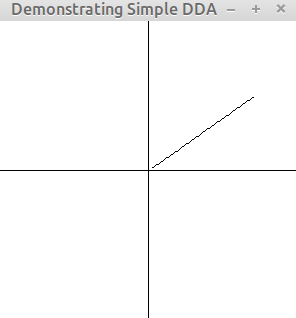
\includegraphics[width=60mm, height=60mm]{line_simple.png}
\caption{Draw Line using Simple DDA in OpenGL \label{overflow}}
\end{figure}

\begin{figure}[ht!]
\centering
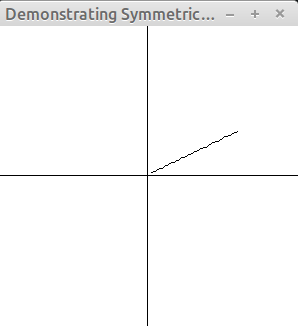
\includegraphics[width=60mm, height=60mm]{line_symmetric.png}
\caption{Draw Line using Symmetric DDA in OpenGL \label{overflow}}
\end{figure}

\begin{figure}[ht!]
\centering
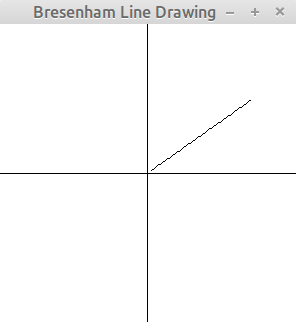
\includegraphics[width=60mm, height=60mm]{line_bresenham.png}
\caption{Draw Line using Bresenham Algorithm in OpenGL \label{overflow}}
\end{figure}

\begin{figure}[ht!]
\centering
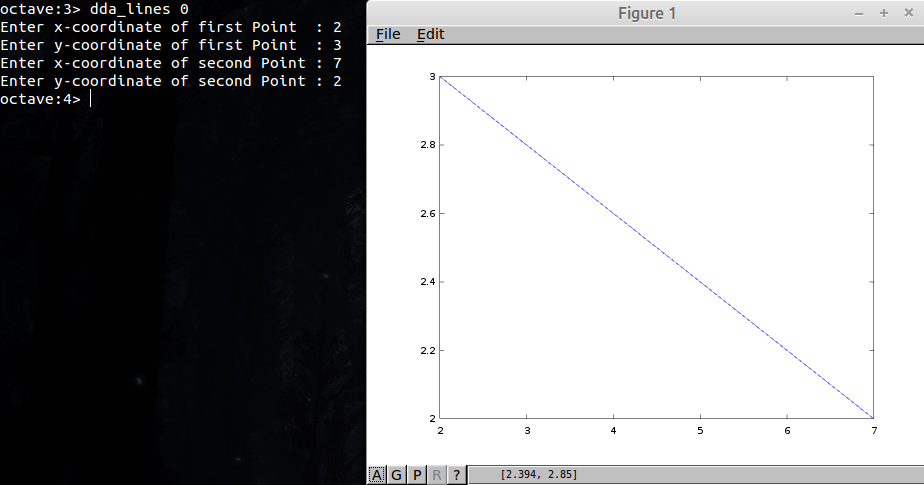
\includegraphics[width=60mm, height=60mm]{line_simple_matlab.png}
\caption{Draw Line using Simple DDA in Matlab \label{overflow}}
\end{figure}

\begin{figure}[ht!]
\centering
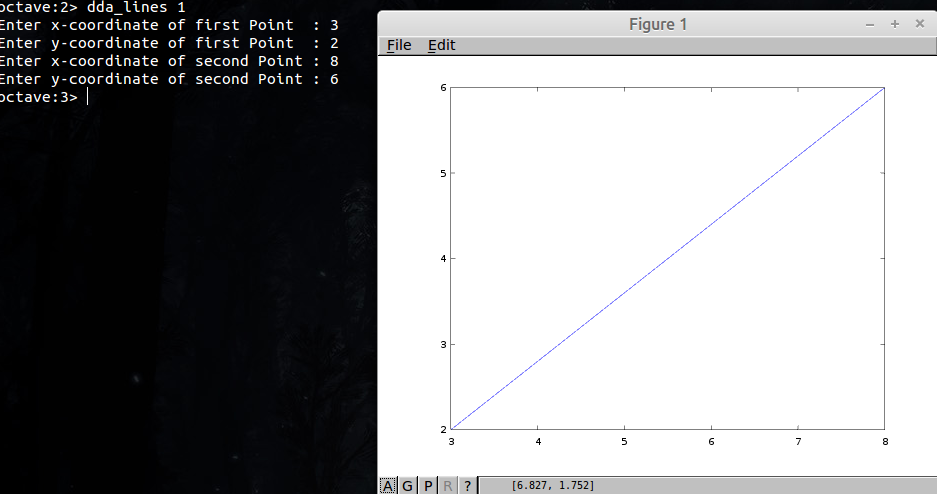
\includegraphics[width=60mm, height=60mm]{line_symmetric_matlab.png}
\caption{Draw Line using Symmetric DDA in  Matlab \label{overflow}}
\end{figure}

\begin{figure}[ht!]
\centering
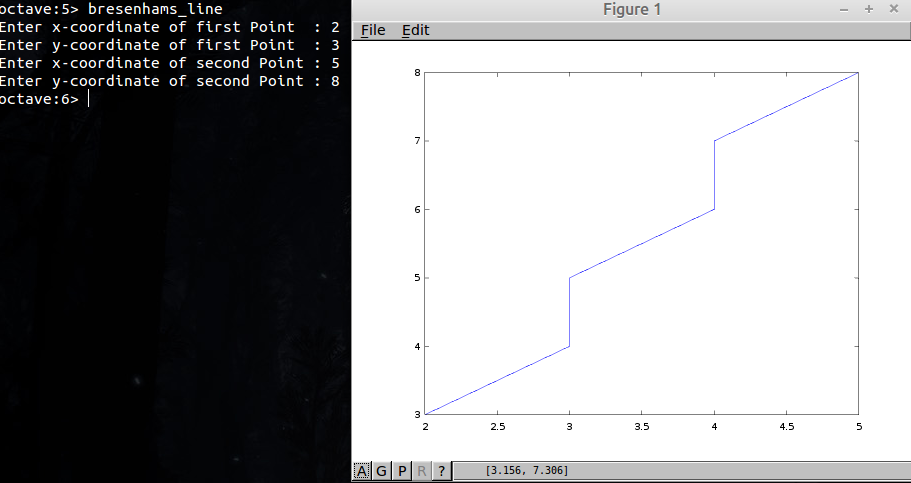
\includegraphics[width=60mm, height=60mm]{line_bresenham_matlab.png}
\caption{Draw Line using Bresenham Algorithm in  Matlab \label{overflow}}
\end{figure}

\end{document}
